\section{Desarrollo}

\subsection{Hardware}
\begin{frame}
\frametitle{Desarrollo}
\framesubtitle{Hardware}
\footnotesize 
\begin{wrapfigure}{r}{0.45\linewidth}
	\centering
	\caption{ESP32 creado en proteus [Imagen Propia]}
	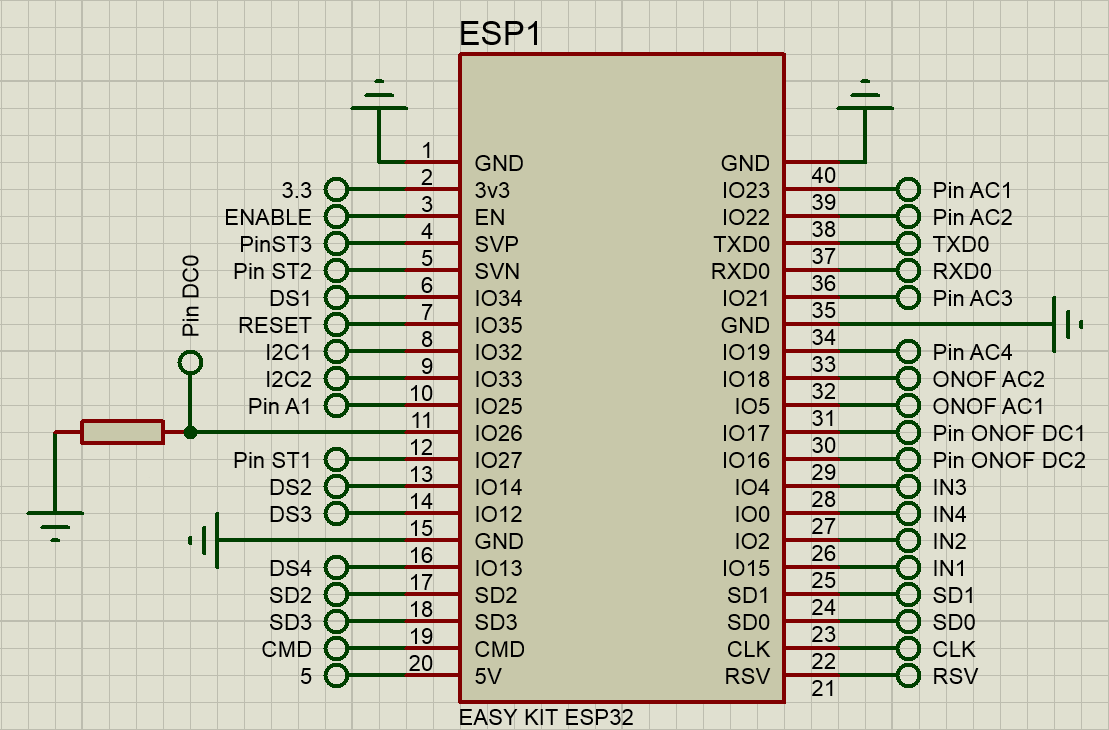
\includegraphics[width=0.7\linewidth]{Imagenes/ESP32}	
	\label{fig:esp32}
\end{wrapfigure}
El prototipo para Smart House tiene por objetivo monitorear el entorno de aplicación y controlarlo por medio de mecanismos como motores o dispositivos de iluminación, razón por la cual está equipada con etapas de potencia de corriente alterna y directa, etapa de adquisición de datos, entre otras características que permitan cumplir con los objetivos planteados.\newline 

El prototipo fue diseñado en el software Proteus, desde el esquemático hasta la placa de circuito impreso (PCB), en la figura \ref{fig:esp32} se observa el esquematico de la tarjeta ESP32 construido junto con su distribución de pines, además de sus conexiones correspondientes dentro de este programa. El prototipo está separado en dos secciones, la etapa de potencia AC y la etapa DC, en la última, se encuentra la mayor parte de circuitos que funcionan con corriente directa.

\end{frame}

\subsubsection{Alimentacion}
\begin{frame}
\frametitle{Desarrollo}
\framesubtitle{Hardware | \emph{Alimentación}}
	\textbf{Corriente alterna (AC):}
		El prototipo recibe el voltaje directamente de la red eléctrica a la que se encuentra conectado el entorno de aplicación, el cual está pensado para una habitación dentro de una Smart House.\newline
		
		\begin{wrapfigure}{r}{0.5\linewidth}
			\centering
			\caption{Modulo conversor DC-DC. Tomado de: \cite{DCDC}}
			\label{fig:DCDC}
			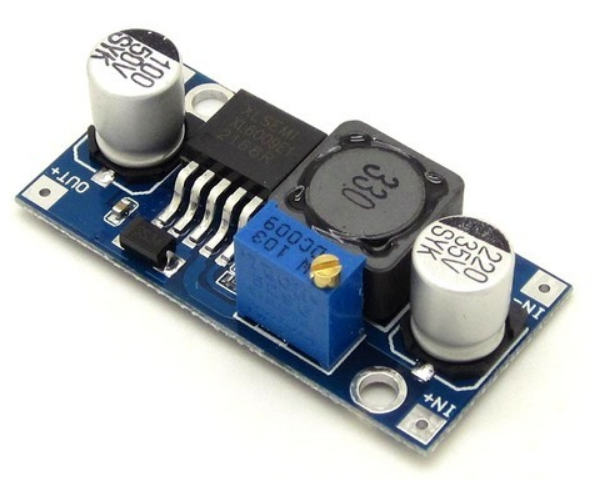
\includegraphics[width=0.5\linewidth]{Imagenes/DCDC}
		\end{wrapfigure}
	\textbf{Corriente directa (DC):}
		Para la alimentación DC del circuito, se hace uso de un conversor AC-DC que regula el voltaje de la red eléctrica a 12V DC, con los cuales se manejara la etapa de potencia DC, además de ser usados por dos modulos conversores DC-DC.\\

\end{frame}
	
\subsubsection{Entradas}

\begin{frame}[t]
\frametitle{Desarrollo}
\framesubtitle{Hardware | \emph{Entradas}}	

\textbf{Sensores:}
		El prototipo viene equipado con una etapa de adquisición de datos con capacidad entre 7 a 134 sensores, pues posee una entrada I2C, ampliando el número de dispositivos conectados, lo cual también permitiría adicionar tareas más específicas en escenarios que lo requieran.\newline
		
		Con la finalidad de realizar pruebas del prototipo, se hacen uso de 5 sensores para medir magnitudes y situaciones en el entorno, tal como calidad del aire, temperatura, humedad, luz visible, movimiento y presencia de lluvia, debido a que estas medidas o estados se encuentran en casi cualquier ambiente. 
\end{frame}

\begin{frame}
\frametitle{Desarrollo}
\framesubtitle{Hardware | \emph{Entradas}}	

		\begin{wrapfigure}{r}{0.5\linewidth}
			\centering
			\caption{Entrada de sensores[Imagen Propia]}
			\label{fig:SVS}
			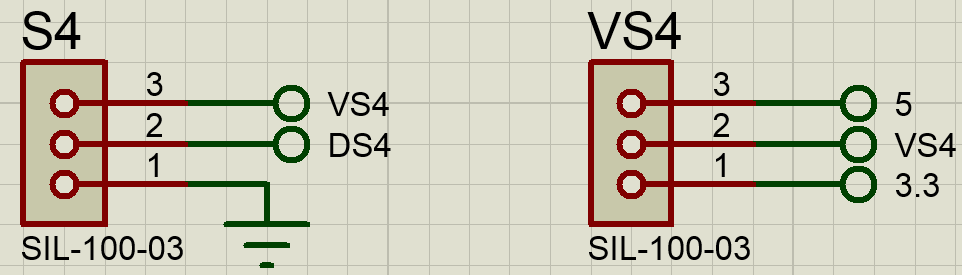
\includegraphics[width=0.7\linewidth]{Imagenes/SVS}
		\end{wrapfigure}
		Teniendo en cuenta que el ESP32 funciona en voltajes lógicos de 3.3V, se tienen 4 entradas de sensores directamente conectados a los pines de la tarjeta, con la capacidad de cambiar el voltaje de alimentación para 3 de ellos, como se muestra en la figura \ref{fig:SVS}, pues en el mercado se encuentran sensores que manejan voltajes de alimentación ya sea de 3.3V o 5V, mientras que la cuarta entrada se encuentra alimentada con 5V, ya que tiene un uso específico en las pruebas para el sensor de calidad de aire, esta viene acondicionada con un diodo zener en contraposición, para evitar que la tarjeta ESP32 tenga un voltaje de entrada superior a 3.3V.\\
\end{frame}

\begin{frame}
\frametitle{Desarrollo}
\framesubtitle{Hardware | \emph{Entradas}}

		Las tres entradas para sensores de estado (ST1, ST2, ST3), a diferencia de las demás, se encuentran conectadas a pines de la tarjeta que no presentan resistencia de pull down por software, por ello se agregan estas al sistema, tal como se observa en la figura \ref{fig:ST}.\\
	
		\begin{figure}
			\centering
			\caption{Entrada para sensores con resistencia de pull down[Imagen Propia]}
			\label{fig:ST}
			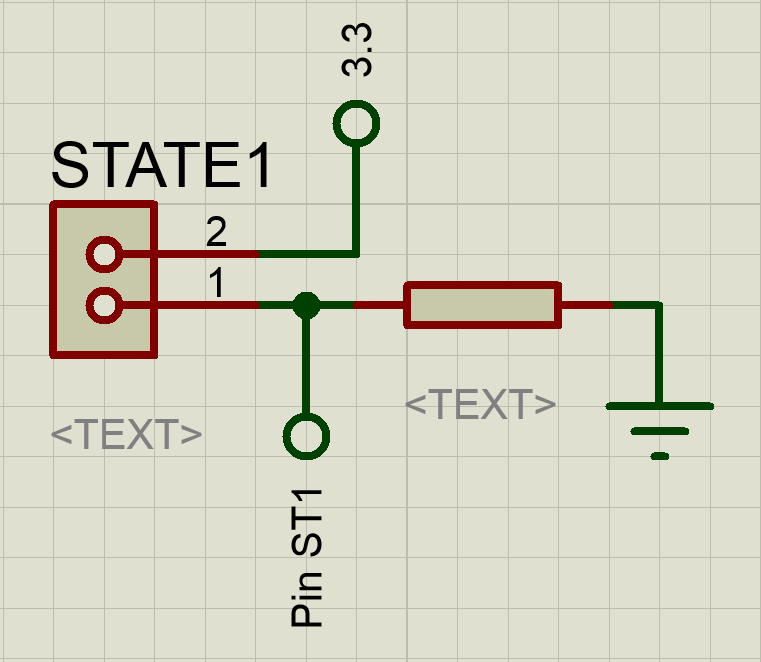
\includegraphics[width=0.35\linewidth]{Imagenes/ST}
		\end{figure}		

\end{frame}

\begin{frame}[t]
\frametitle{Desarrollo}
\framesubtitle{Hardware | \emph{Otras Entradas}}

	\textbf{Calibración de audio:}
		Para calibrar la salida audible se hace uso de una resistencia variable (Potenciometro), el cual permite regular el voltaje de entrada al circuito de amplificación mostrado en la figura \ref{fig:AUD}; este será descrito en el presente capitulo en la sección de salidas del hardware.\newline
		
	\textbf{Botón enable:}
		Presionando el botón enable se reinicia la tarjeta ESP32, junto con su firmware.\newline
		
	\textbf{Botón reset:}
		Presionando el botón reset se borran las credenciales ingresadas para la conexión del ESP32 a la red wifi.\newline

\end{frame}

	\subsubsection{Salidas}
\begin{frame}
	\frametitle{Desarrollo}
	\framesubtitle{Hardware | \emph{Etapa de Potencia AC}}
		Se encuentra diseñada a una potencia de 2000W en un total de seis cargas, cuatro de ellas cuentan con un circuito para el control por ángulo de fase, como se observa en la figura \ref{fig:CAC1}, con una capacidad individual de 500W, gracias a el TRIAC BTA26600, el cual soporta una corriente máxima de 25A. Con el fin de proteger el ESP32, se hace uso de optoacopladores MOC3021, debido a su funcionalidad para aislar circuitos de forma óptica.
		\begin{figure}
			\centering
			\caption{Control por angulo de fase [Imagen Propia]}
			\label{fig:CAC1}
			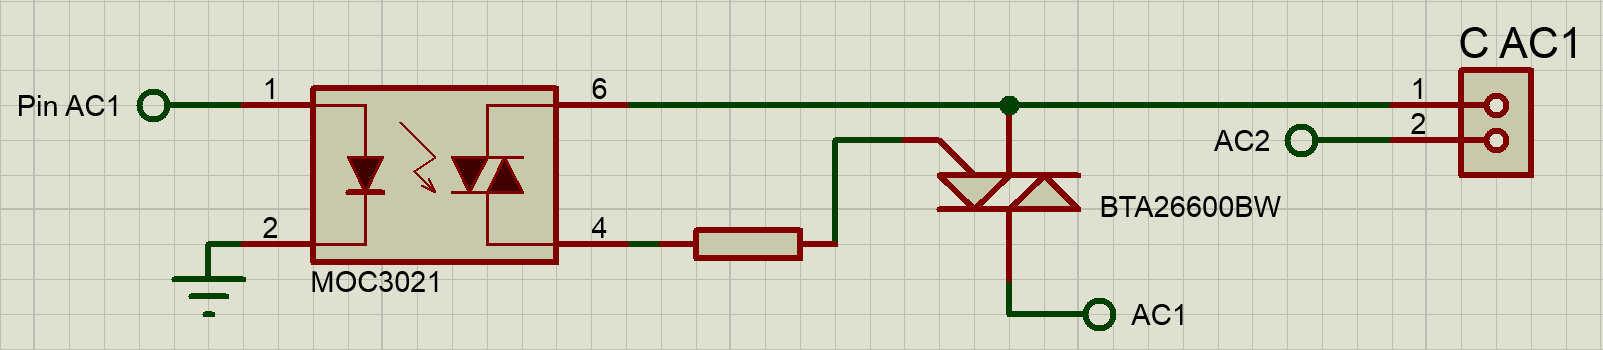
\includegraphics[width=0.8\linewidth]{Imagenes/CAC1}
		\end{figure}
	
\end{frame}
\begin{frame}
\frametitle{Desarrollo}
\framesubtitle{Hardware | \emph{Etapa de Potencia AC}}
\small	
		Las dos cargas restantes corresponden a un sistema de encendido y apagado, cuyo funcionamiento se basa en un relevador SRA-05VDC-CL activado a 5V por medio de un transistor BJT como switch, gracias a este relé, las salidas tienen capacidad de hasta 200W cada una, en la figura \ref{fig:ONOFAC} se observa el circuito diseñado en proteus. Para proteger el ESP32 el prototipo se vale de ese dispositivo, puesto que presenta un aislamiento magnético por la naturaleza de su operación.
		\begin{figure}
			\centering
			\caption{Interruptor para cargas AC [Imagen Propia]}
			\label{fig:ONOFAC}
			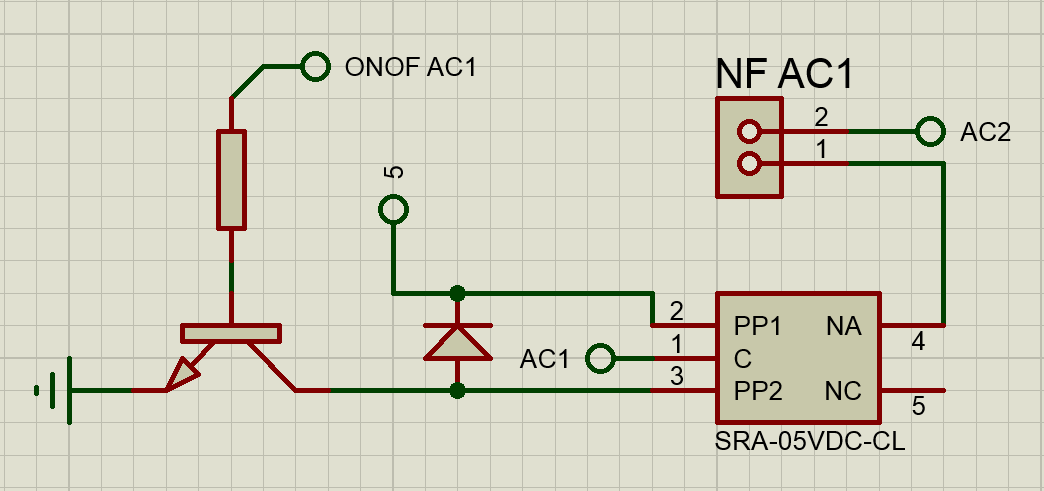
\includegraphics[width=0.45\linewidth]{Imagenes/ONOFAC}
		\end{figure}
\end{frame}

\begin{frame}
\frametitle{Desarrollo}
\framesubtitle{Hardware | \emph{Detector de Cruce por Cero}}
\small
		Dentro de la etapa AC se encuentra el detector de cruce por cero, el cual cuenta con un fototransistor 4N25, debido a su alta capacidad de aislamiento, tomando la onda rectificada completa y pasándola a un nivel lógico de 3.3V, esta parte del circuito se observa en la figura \ref{fig:DC01}; para que la señal sea más confiable se hace uso de un Schmitt-Trigger CD40106, valiéndose de la histéresis de voltaje garantizando que la señal de salida sea poco susceptible al ruido \cite{DC0}.\\
		
		\begin{figure}
			\centering
			\caption{Detector de cruce por cero [Imagen Propia]}
			\label{fig:DC01}
			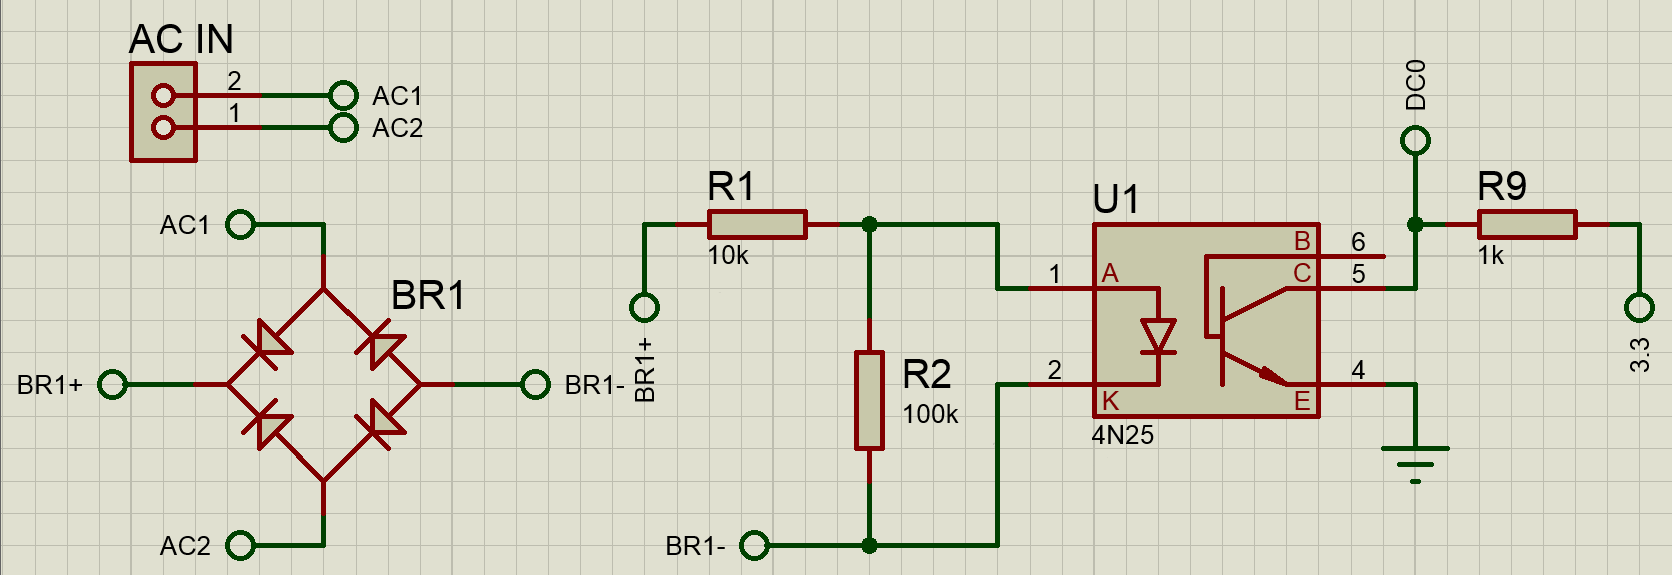
\includegraphics[width=0.65\linewidth]{Imagenes/DC01}
		\end{figure}
\end{frame}

\begin{frame}
\frametitle{Desarrollo}
\framesubtitle{Hardware | \emph{Etapa DC}}
\footnotesize 
\begin{wrapfigure}{r}{0.4\linewidth}
	\centering
	\caption{\scriptsize Puente h para control de motores DC [Imagen Propia]}
	\label{fig:CDC}
	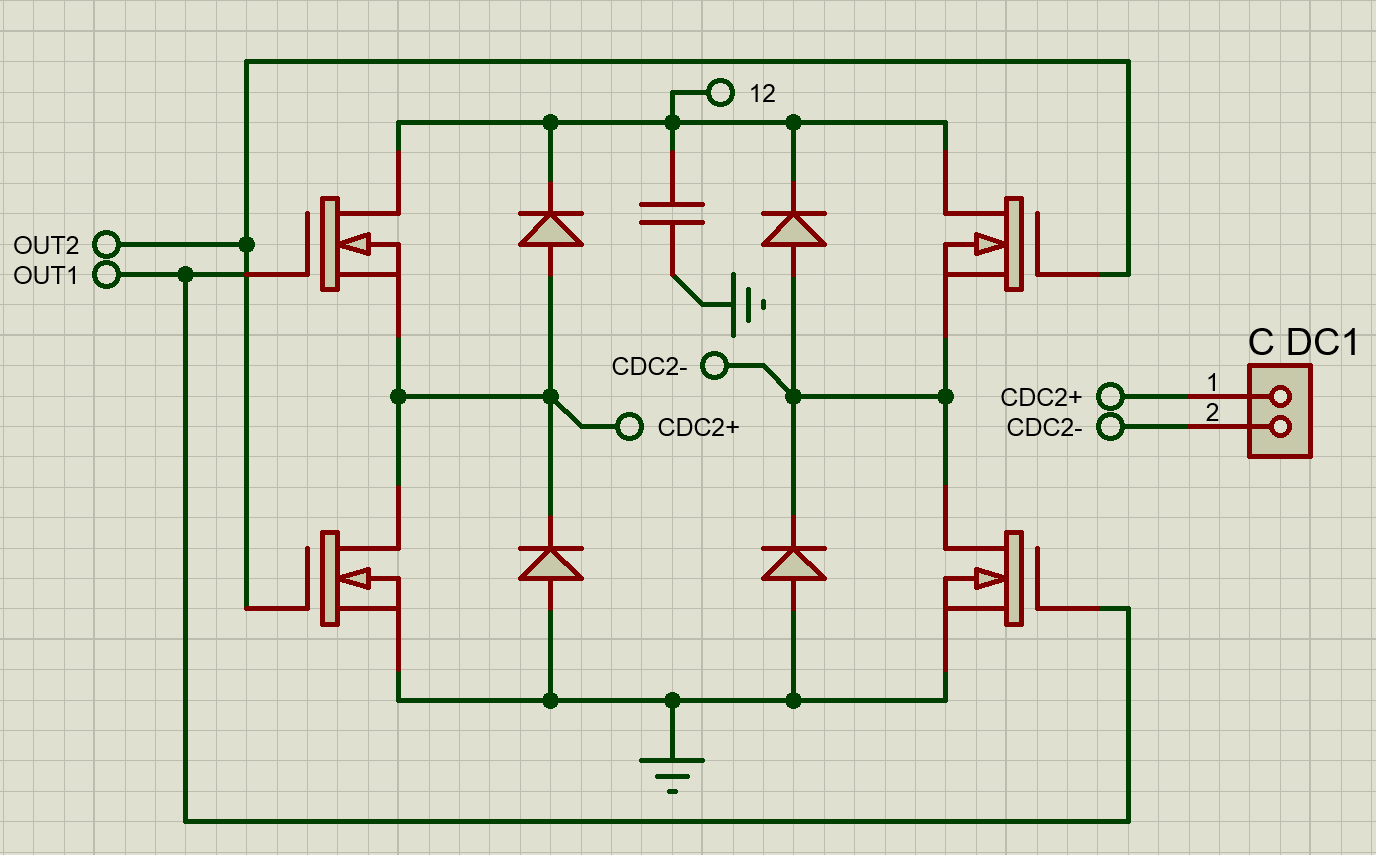
\includegraphics[width=0.8\linewidth]{Imagenes/CDC}
\end{wrapfigure}
		Esta etapa cuenta con cuatro salidas de control diseñadas para cargas de 12V, de las cuales, dos de ellas tienen un enfoque a motores, puesto que está equipada con control de velocidad a base de PWM e inversión de giro con un puente h usando transistores mosfet IRLZ44N; el puente h se encuentra controlado por un circuito integrado L293D, que garantiza un voltaje Vgs adecuado para la correcta activación del los transistores; este circuito se muestra en la figura \ref{fig:CDC}.\cite{IRL}.\newline
		
		Las dos salidas restantes también cuentan con mosfet IRLZ44N, y su control igualmente es a base de PWM, mas no permite realizar la inversión de giro, por lo cual se enfoca a dispositivos como lámparas LEDs.\\
	
\end{frame}

\begin{frame}
\frametitle{Desarrollo}
\framesubtitle{Hardware | \emph{Salida Audible}}

\begin{wrapfigure}{r}{0.4\linewidth}
	\centering
	\caption{Circuito tipico para el LM386 [Imagen Propia]}
	\label{fig:AUD}
	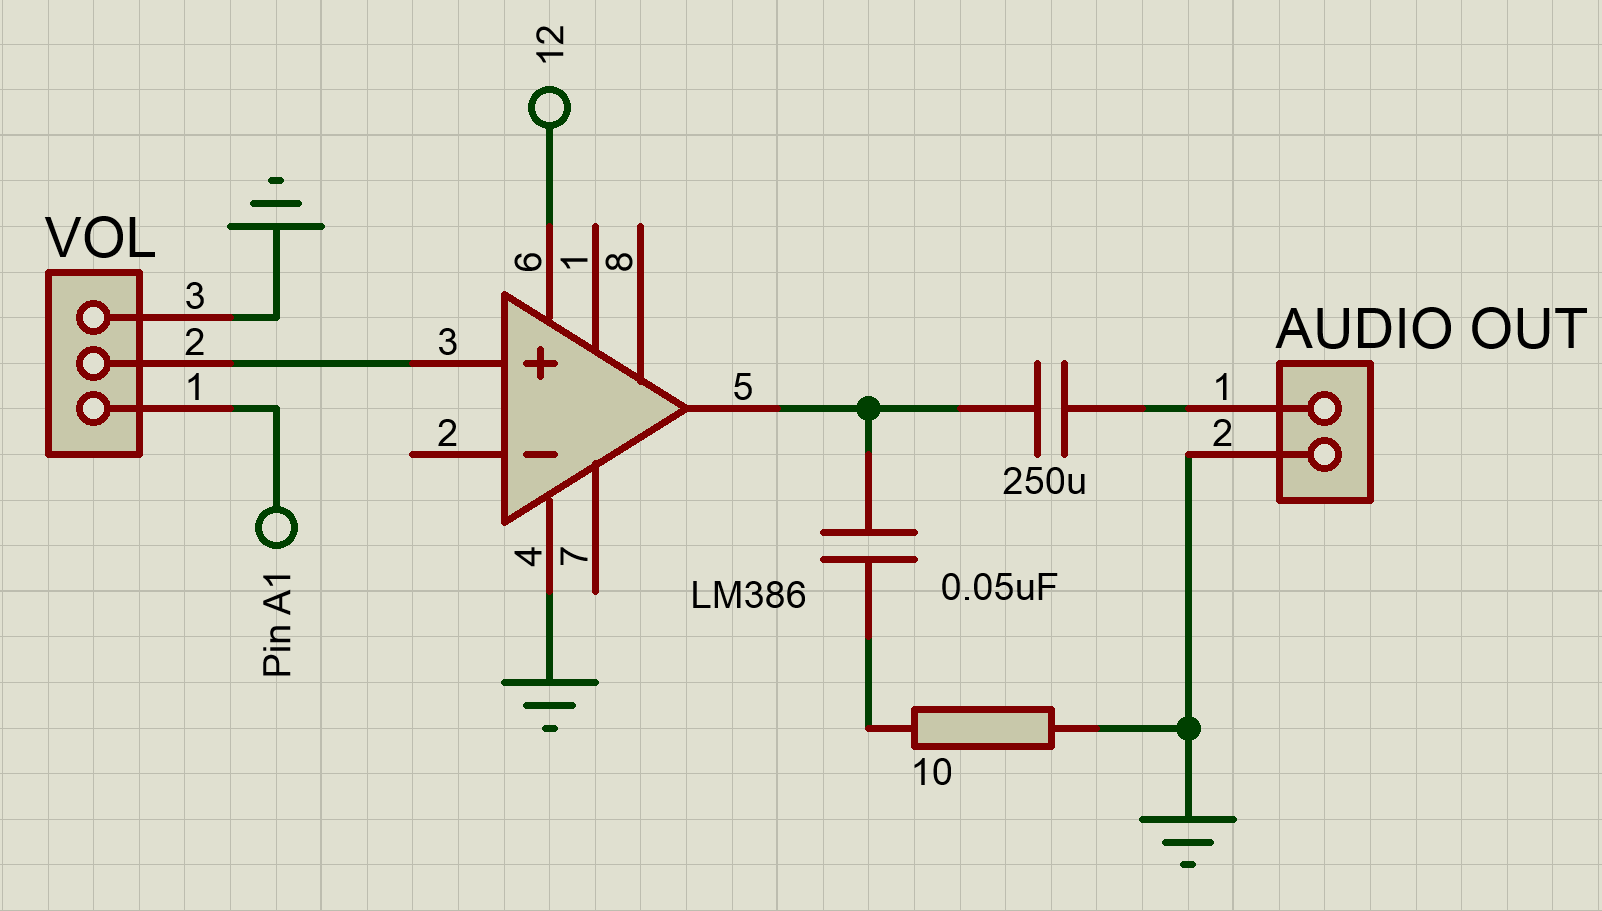
\includegraphics[width=0.8\linewidth]{Imagenes/AUD}
\end{wrapfigure}
		Está diseñada para emitir sonidos a una sola frecuencia, o sonido mono estéreo, caso dado cuando se activa una regla programada en la aplicación web, enfocada a las cargas de encendido y apagado, tanto de la etapa de potencia AC como la etapa DC.\newline
		
		El circuito utilizado para la salida audible está basado en el amplificador de audio LM386, implementando el esquema típico de aplicación ilustrado en su datasheet \cite{LM386}, en la figura \ref{fig:AUD} se observa implementado en el software proteus.\\
\end{frame}		
				
\subsection{Firmware}

\begin{frame}
\frametitle{Desarrollo}
\framesubtitle{Firmware}
\begin{wrapfigure}{r}{0.5\linewidth}
	\centering
	\caption{ESP-IDF. Tomado de: \cite{ES}}
	\label{fig:what-you-need}
	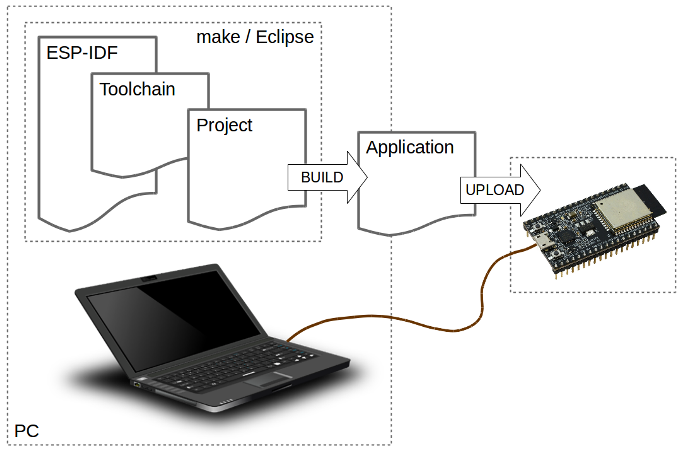
\includegraphics[width=0.7\linewidth]{Imagenes/what-you-need}
\end{wrapfigure}
El firmware se desarrolla sobre el SDK oficial de Espressif Systems ESP-IDF, para el desarrollo de la aplicación es necesario contar con los requisitos que se observan en la figura \ref{fig:what-you-need}. Esta característica del sistema incluye un kernel de tiempo real llamado FreeRTOS, al ser un RTOS, las funciones se definen mediante tareas, entonces cada funcionalidad de la tarjeta o grupo de funcionalidades se desarrolla en una o varias tareas que realicen las acciones adecuadas.\\
\end{frame}

\begin{frame}
\frametitle{Desarrollo}
\framesubtitle{Firmware}

Sobre el firmware se desarrollan los siguientes temas:

\begin{itemize}
	\item Tareas
	\item GPIO
	\item ADC,DAC
	\item HTTP Request
	\item Hora de Red
	\item Timers
	\item I2C
	\item PWM
	\item Interrupciones
\end{itemize}

\end{frame}

\subsection{Software}

\begin{frame}
\frametitle{Desarrollo}
\framesubtitle{Software}
\small
Se desarrolla una aplicación web, la cual se encarga de ejecutar la gestión entre el usuario y la tarjeta. De este modo, se usa un patrón de arquitectura Modelo-Vista-Controlador (MVC), siendo este realmente útil ya que separa la lógica de negocio de la interfaz de usuario, incrementando la reutilización y flexibilidad, además de la escalabilidad de ambos aspectos por separado, dicho esto, la aplicación cuenta con diferentes modelos, controladores y vistas \cite{MVC1}. La función de cada parte de esta arquitectura se puede observar en la figura \ref{fig:mvc}.
\begin{figure}[H]
	\centering
	\caption{Modelo-Vista-Controlador [Imagen Propia]}
	\label{fig:mvc}
	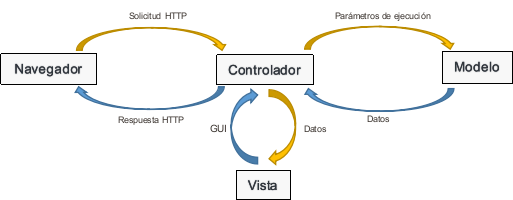
\includegraphics[width=0.55\linewidth]{Imagenes/MVC}
\end{figure}

\end{frame}

\begin{frame}[t]
\frametitle{Desarrollo}
\framesubtitle{Software}
\small
Además, el framework Laravel hace uso de un ORM (Mapeo Objeto-Relacional) llamado Eloquent. Esta es una forma de mapear los datos que se encuentran en la base de datos a objetos de PHP y viceversa, esto facilita el uso de diferentes gestores de bases de datos como MySQL, SQLite, entre otras, ya que todas las consultas estan en PHP y el ORM ya se encarga del mapeo a los comandos SQL como se observa en la figura \ref{fig:orm}. Eloquent usa los modelos para enviar y recibir información de la base de datos\cite{Eloq}.\\

\begin{figure}[H]
	\centering
	\caption[ORM]{ORM [Imagen Propia]}
	\label{fig:orm}
	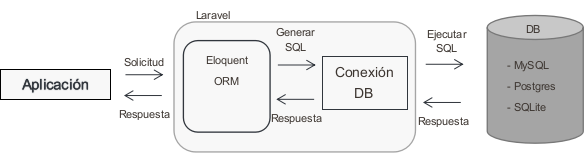
\includegraphics[width=0.7\linewidth]{Imagenes/ORM}
\end{figure}

\end{frame}

\subsection{Prueba Beta}

\begin{frame}[t]
\frametitle{Desarrollo}
\framesubtitle{Prueba Beta Cerrada}

Esta prueba se desarrolla en el entorno del cliente o usuario, arrojando resultados sobre las funcionalidades provistas para el software, además de dar la aceptación por parte del cliente si el producto funciona de manera adecuada o esperada \cite{PB}. Con el fin de realizar dicha verificación se analizan los objetivos a cumplir y los alcances, por lo tanto se separan los casos de prueba con el propósito de formular las preguntas que deben contestar las personas.\newline

\begin{itemize}

\item Prueba de conectividad de la tarjeta

\item Prueba de la Aplicación Web
\end{itemize}

\end{frame}